\section{Code Quality}
Once the code is in Conventional SSA, destructing it is straightforward, which solves the correctness problem. To improve the code however, it
is important to remove as many copies as possible. This can be treated
with classic coalescing as conventional SSA allows to get rid of \phifuns: the set of variables of a SSA web can be coalesced leading to a single non-SSA variable; liveness and
interferences can then be defined as for regular code (with parallel copies). An interference graph (as depicted in Figure~\ref{fig:alternative_ssa_destruction:ex_lost_c}) can be used. A plain edge between two nodes (e.g. between $x_2$ and $x_3$) materialize the presence of an interference between the two corresponding variables (e.g. between $x_2$ and $x_3$), i.e. expressing the fact that they cannot be coalesced and share the same resource. A dashed edge between two nodes materializes an affinity between the two corresponding variables, i.e. the presence of a copy (e.g. between $x_2$ and $u_0$) that could be removed by their coalescing.

This process is illustrated by Figure~\ref{fig:alternative_ssa_destruction:ex_lost}: the isolation of the \phifun leads to inserting the three copies that respectively define $u_1$ and $u_2$ and uses $u_0$; the corresponding \phiweb  $\{u_0, u_1, u_2\}$ is coalesced into a representative variable $u$; according to the interference graph of Figure~\ref{fig:alternative_ssa_destruction:ex_lost_c}, $x_1$, $x_5$ can then be coalesced with $u$ leading to the code of Figure~\ref{fig:alternative_ssa_destruction:ex_lost_d}.

If the goal is not to destruct SSA completely but remove as many copies as possible while maintaining the conventional property, liveness of \phifun operands should reproduce the behavior of the corresponding non-SSA code as if the variables of the \phiweb were coalesced all together. The semantic of the \phiop in the so called \emph{multiplexing} mode
fits the requirements. The corresponding interference graph on our example is depicted in Figure~\ref{fig:alternative_ssa_destruction:ex_lost_c_cssa}.


\begin{definition}[multiplexing mode]
Let a \phifun $B_0:a_0=\phi(B_1:a_1,\dots,B_n:a_n)$ be in \emph{multiplexing} mode, then its liveness follows the following semantic: its \defop is considered to be at the entry of $B_0$, in other words variable $a_0$ is live-in of $B_0$; its \useops are at the exit\index{basic-block exit} of the corresponding predecessor basic-blocks, in other words variable $a_i$ for $i>0$ is live-out of basic-block $B_i$.
\end{definition}


\begin{figure}[H]
\subfloat[Lost-copy problem]{
  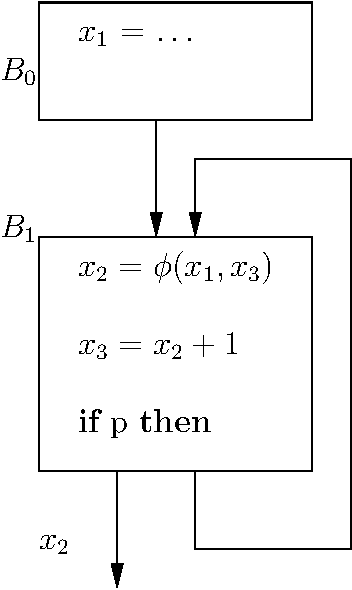
\includegraphics[width=0.20\textwidth]{lost.pdf}
}
\hfill
\subfloat[Corresponding CSSA code]{
  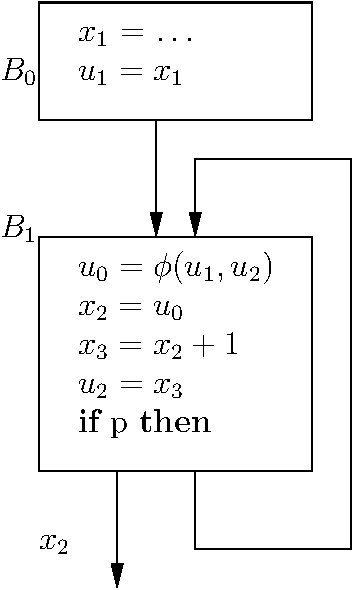
\includegraphics[width=0.20\textwidth]{lost2.pdf}
}
\hfill
\begin{minipage}[b]{0.2\textwidth}
  \subfloat[\label{fig:alternative_ssa_destruction:ex_lost_c_cssa}Interferences under CSSA]{
    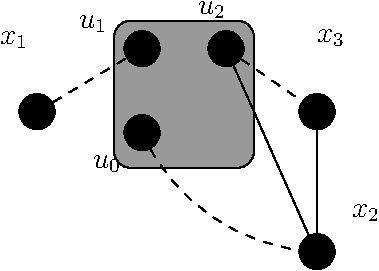
\includegraphics[width=\textwidth]{lost-graph-cssa.pdf}
}\\
  \subfloat[\label{fig:alternative_ssa_destruction:ex_lost_c}Interferences and coalescing]{
    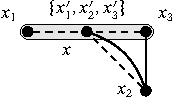
\includegraphics[width=\textwidth]{lost-graph.pdf}
  }
\end{minipage}
\hfill
\subfloat[\label{fig:alternative_ssa_destruction:ex_lost_d}After copy optimization]{
  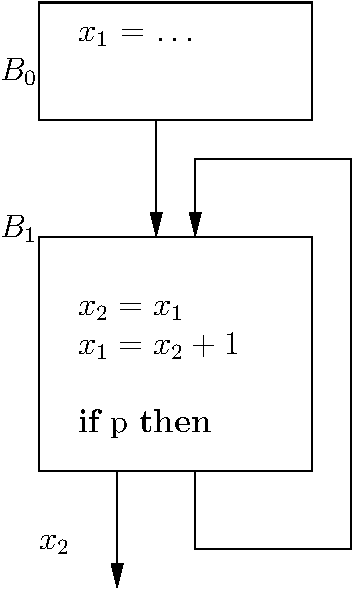
\includegraphics[width=0.20\textwidth]{lost3.pdf}
}
\caption{Out-of-SSA translation for the lost-copy problem.\label{fig:alternative_ssa_destruction:ex_lost}}
\end{figure}

As already mentioned 
